\input{header_slides.tex}

\begin{document}

\title
[A generative model for urban firm networks]{A generative model for urban firm networks}
\author[Raimbault \and Zdanowska]{J.~Raimbault$^{1,2,3\ast}$ \and N. Zdanowska$^{1,3}$\\\medskip
$^{\ast}$\texttt{n.zdanowska@ucl.ac.uk}
}

\institute[UCL]{$^{1}$Center for Advanced Spatial Analysis, University College London\\
$^{2}$UPS CNRS 3611 Complex Systems Institute Paris\\
$^{3}$UMR CNRS 8504 G{\'e}ographie-cit{\'e}s
}




\date[24/09/2020]{NetSci 2020\\
Session 12F: Diffusion\\
September 24th, 2020
}

\frame{\maketitle}

\section{Introduction}


\sframe{Urban firm networks}{


General framework:

\medskip

\begin{itemize}
\item Cities as cross-overs of socio-economic interactions           \cite{castells1996information}
    \item Networks as the new social morphology of societies \cite{castells2000networksociety}, giving rise to network economies \cite{sassen1991global} 
    \item Emergence of an interconnected world city network as a crucial feature of globalisation \cite{taylor2001specification}  
    \item Interurban interactions between firms as one of the most representative of economic trends \cite{martinus2018global}
    
\end{itemize}

\bigskip

}

\sframe{An evolutionary approach to Urban Systems}{

\begin{itemize}
    \item Evolutionary Theory of Urban Systems \cite{pumain1997pour} \cite{pumain2006villes}
    \item Adaptive cycles and diffusion of innovation \cite{Hagerstrand1968Innovation}
    \item Path dependence \cite{martin2006path} \cite{pumain2012urban}
    \item Selection and emerging structures of systems 
    \item Evolutionary models for urban systems dynamics: \cite{favaro2011gibrat} \cite{cottineau2015growing} \cite{schmitt2015half} \cite{raimbault2018calibration} \cite{raimbault2018indirect} \cite{Raimbault_2020}
\end{itemize}

}

\sframe{Urban firm linkages and geo-economic processes}{

Assumptions:

\medskip

\begin{itemize}
    \item Metropolisation \& internationalisation effects
    \item Specialisation-driven factors and drivers of innovation
    \item Macroeconomic exogenous chocs and resilience of urban systems 
\end{itemize}

\bigskip

$\rightarrow$ \textit{How can we capture geographical and economic processes within urban networks of firms with a generative model?}

\medskip

\begin{itemize}
	\item Indirect inference on processes
	\item Includes path-dependency
\end{itemize}

}

\sframe{Contribution}{

We examine the interactions of European cities within firm linkages defined by
corporate ownership links and introduce

\medskip

\begin{itemize}
    \item an empirical analysis of the firm ownership urban network in the European Union, based on the Bureau Van Dijk's AMADEUS database;
    \item a generative network model to simulate the growth of such linkages at urban areas scale;
    \item the model allows us to compare the effect of different factors on the final network structure, which is extensively studied through model sensitivity analysis and exploration;
   \item we calibrate the model on the empirical network and apply it to stylized economic shock scenarios.
\end{itemize}

}

\section{Model}

\sframe{Model rationale}{

$\rightarrow$ Cities are defined by their GDP and their profile regarding the proportion of firms in the different sectors. Links between cities are created in an iterative way, taking into account:

\medskip

    \begin{itemize}
        \item geographical proximity (distance or effective accessibility)
        \item geopolitical proximity (belonging to the same country or single market $\rightarrow$ application to Brexit)
        \item city size (economic size as GDP) 
        \item economic similarity (e.g. cosine distance between sector proximity as done in \cite{2019arXiv190505106C}
        \item previous linkages 
    \end{itemize}

}


\sframe{Formalization}{

Cities characterized by economic size $E_i$ (GDP) and economic structure $S_{ik}$ (probability distribution of firms within $K$ sectors)


\medskip

Starting from an initial network, at each time step, add a fixed number of links randomly, following a probability as a generalized Cobb-Douglas function

\[
     p_{ij} \propto \left(\frac{E_{i}}{E}\right)^{\gamma_O} \cdot \left(\frac{E_{j}}{E}\right)^{\gamma_D} \cdot \left(\frac{w_{ij}}{W}\right)^{\gamma_W} \cdot s\left(S_{ik},S_{jk}\right)^{\gamma_S} \cdot \exp \left(- \frac{d_{ij}}{ d_0}\right) \cdot \exp \left(- \frac{c_{ij}}{c_0}\right)
\]

where $E \textrm{ = } \sum_k E_k$, $W \textrm{ = } \sum_{i,j} w_{ij}$, $s$ is a proximity measure given by cosine similarity, $d_{ij}$ euclidian distance, and $c_{ij}$ a socio-cultural distance

\medskip

\textbf{Model parameters: } $\gamma_O, \gamma_D, \gamma_W, \gamma_S, d_0, c_0$

\medskip

\textbf{Model indicators: } internationalisation (modularity of countries in the network), metropolisation (correlation between weighted degree and city size), optimal modularity, average community size

}


\sframe{Empirical data}{

 \begin{center}
 \includegraphics[width=0.7\textwidth]{../../figures/Fig2.png}
 \end{center}
 
 \footnotesize
 
  \textit{Map of network communities obtained by modularity maximisation (European ownership network between Functional Urban Areas, constructed from the AMADEUS database).}

}

\sframe{Statistical models}{



Most general spatial interaction model with fixed effects:

\begin{equation}
\log w_{ij} \textrm{ = } \log d_{ij} \textrm{ + } \log T_i \textrm{ + } \log T_j \textrm{ + } \log s_{ij} \textrm{ + } \alpha_{c_i,c_j} \textrm{ + } \varepsilon_{ij}
\end{equation}

\bigskip
\bigskip

\resizebox{\linewidth}{!}{
\begin{tabular}{|l|c|c|c|c|c|}
\hline
Model  & (1) & (2) & (3) & (4) & (5 - Poisson GLM) \\ 
\hline
$\log(d_{ij})$ &      -0.06** (0.03) &   -0.11** (0.05)  & -0.41*** (0.02)  & -0.35*** (0.04)  &  -0.26*** ($5\cdot 10^{-6}$) \\
$\log(T_i)$ &   &   & 0.56*** (0.01) &  0.56*** (0.01) & 0.79*** ($2\cdot 10^{-6}$) \\
$\log(T_j)$ &     &   & 0.39*** (0.01) &  0.39*** (0.01) & 0.66***  ($1.5\cdot 10^{-6}$) \\
$\log(s_{ij})$ &     &   &  &  0.19*** (0.07) & 0.53*** ($9\cdot 10^{-6}$)  \\
Countries &    &  28.3\% &   &  26.5\% & 100\% \\
\hline
$R^2$ &       0.00059   &  0.17 & 0.21 &  0.31  &  0.56 \\
MSE & 7.75 & 6.84 & 6.10 & 5.33 & 8.72 \\
AIC &        44304   &  43578  &  42131  & 41917 &   \\
\hline
\end{tabular}
}

}

\begin{frame}[label=setupmain]

\frametitle{Model setup}

\justify
 
\begin{enumerate} 
    \item Simulation on synthetic systems of cities \cite{raimbault2019space}: generation of a continent-scale urban system with stylized order of magnitude corresponding to Europe (urban hierarchy, countries, industrial sector distributions - \hyperlink{syntheticsetup}{\beamerbutton{Details}})
    \bigskip
    \item Simulation on the European system of cities (AMADEUS data at FUA level)
\end{enumerate}

\end{frame}


\section{Results}

\sframe{Implementation and experiments}{

\footnotesize

\textbf{Implementation}

\begin{itemize}
	\item Model implemented in NetLogo (good compromise interactivity / ergonomy), with fast data structures (matrix/table extensions)
	\item Integrated seamlessly into OpenMOLE \cite{reuillon2013openmole} for model exploration \url{https://openmole.org/}
\end{itemize}

\begin{center}
\includegraphics[width=0.1\linewidth]{../../figuresraw/iconOM.png}
\includegraphics[width=0.4\linewidth]{../../figuresraw/openmole.png}
\end{center}

\medskip

\textbf{Experiments}

\begin{itemize}
	\item One-factor sampling with 100 repetitions to assess statistical properties (good convergence, average sharpe ratios for indicators all larger than 5)
	\item Grid sampling with 20 repetitions for model behavior
	\item Targeted experiment on impact of synthetic hierarchy
	\item Global Sensitivity Analysis \cite{saltelli2008global}
	\item Calibration on real setup with a Genetic Algorithm
	\item Application to economic shocks scenarios
\end{itemize}

}

\sframe{Simulation of urban networks}{


 \begin{center}
 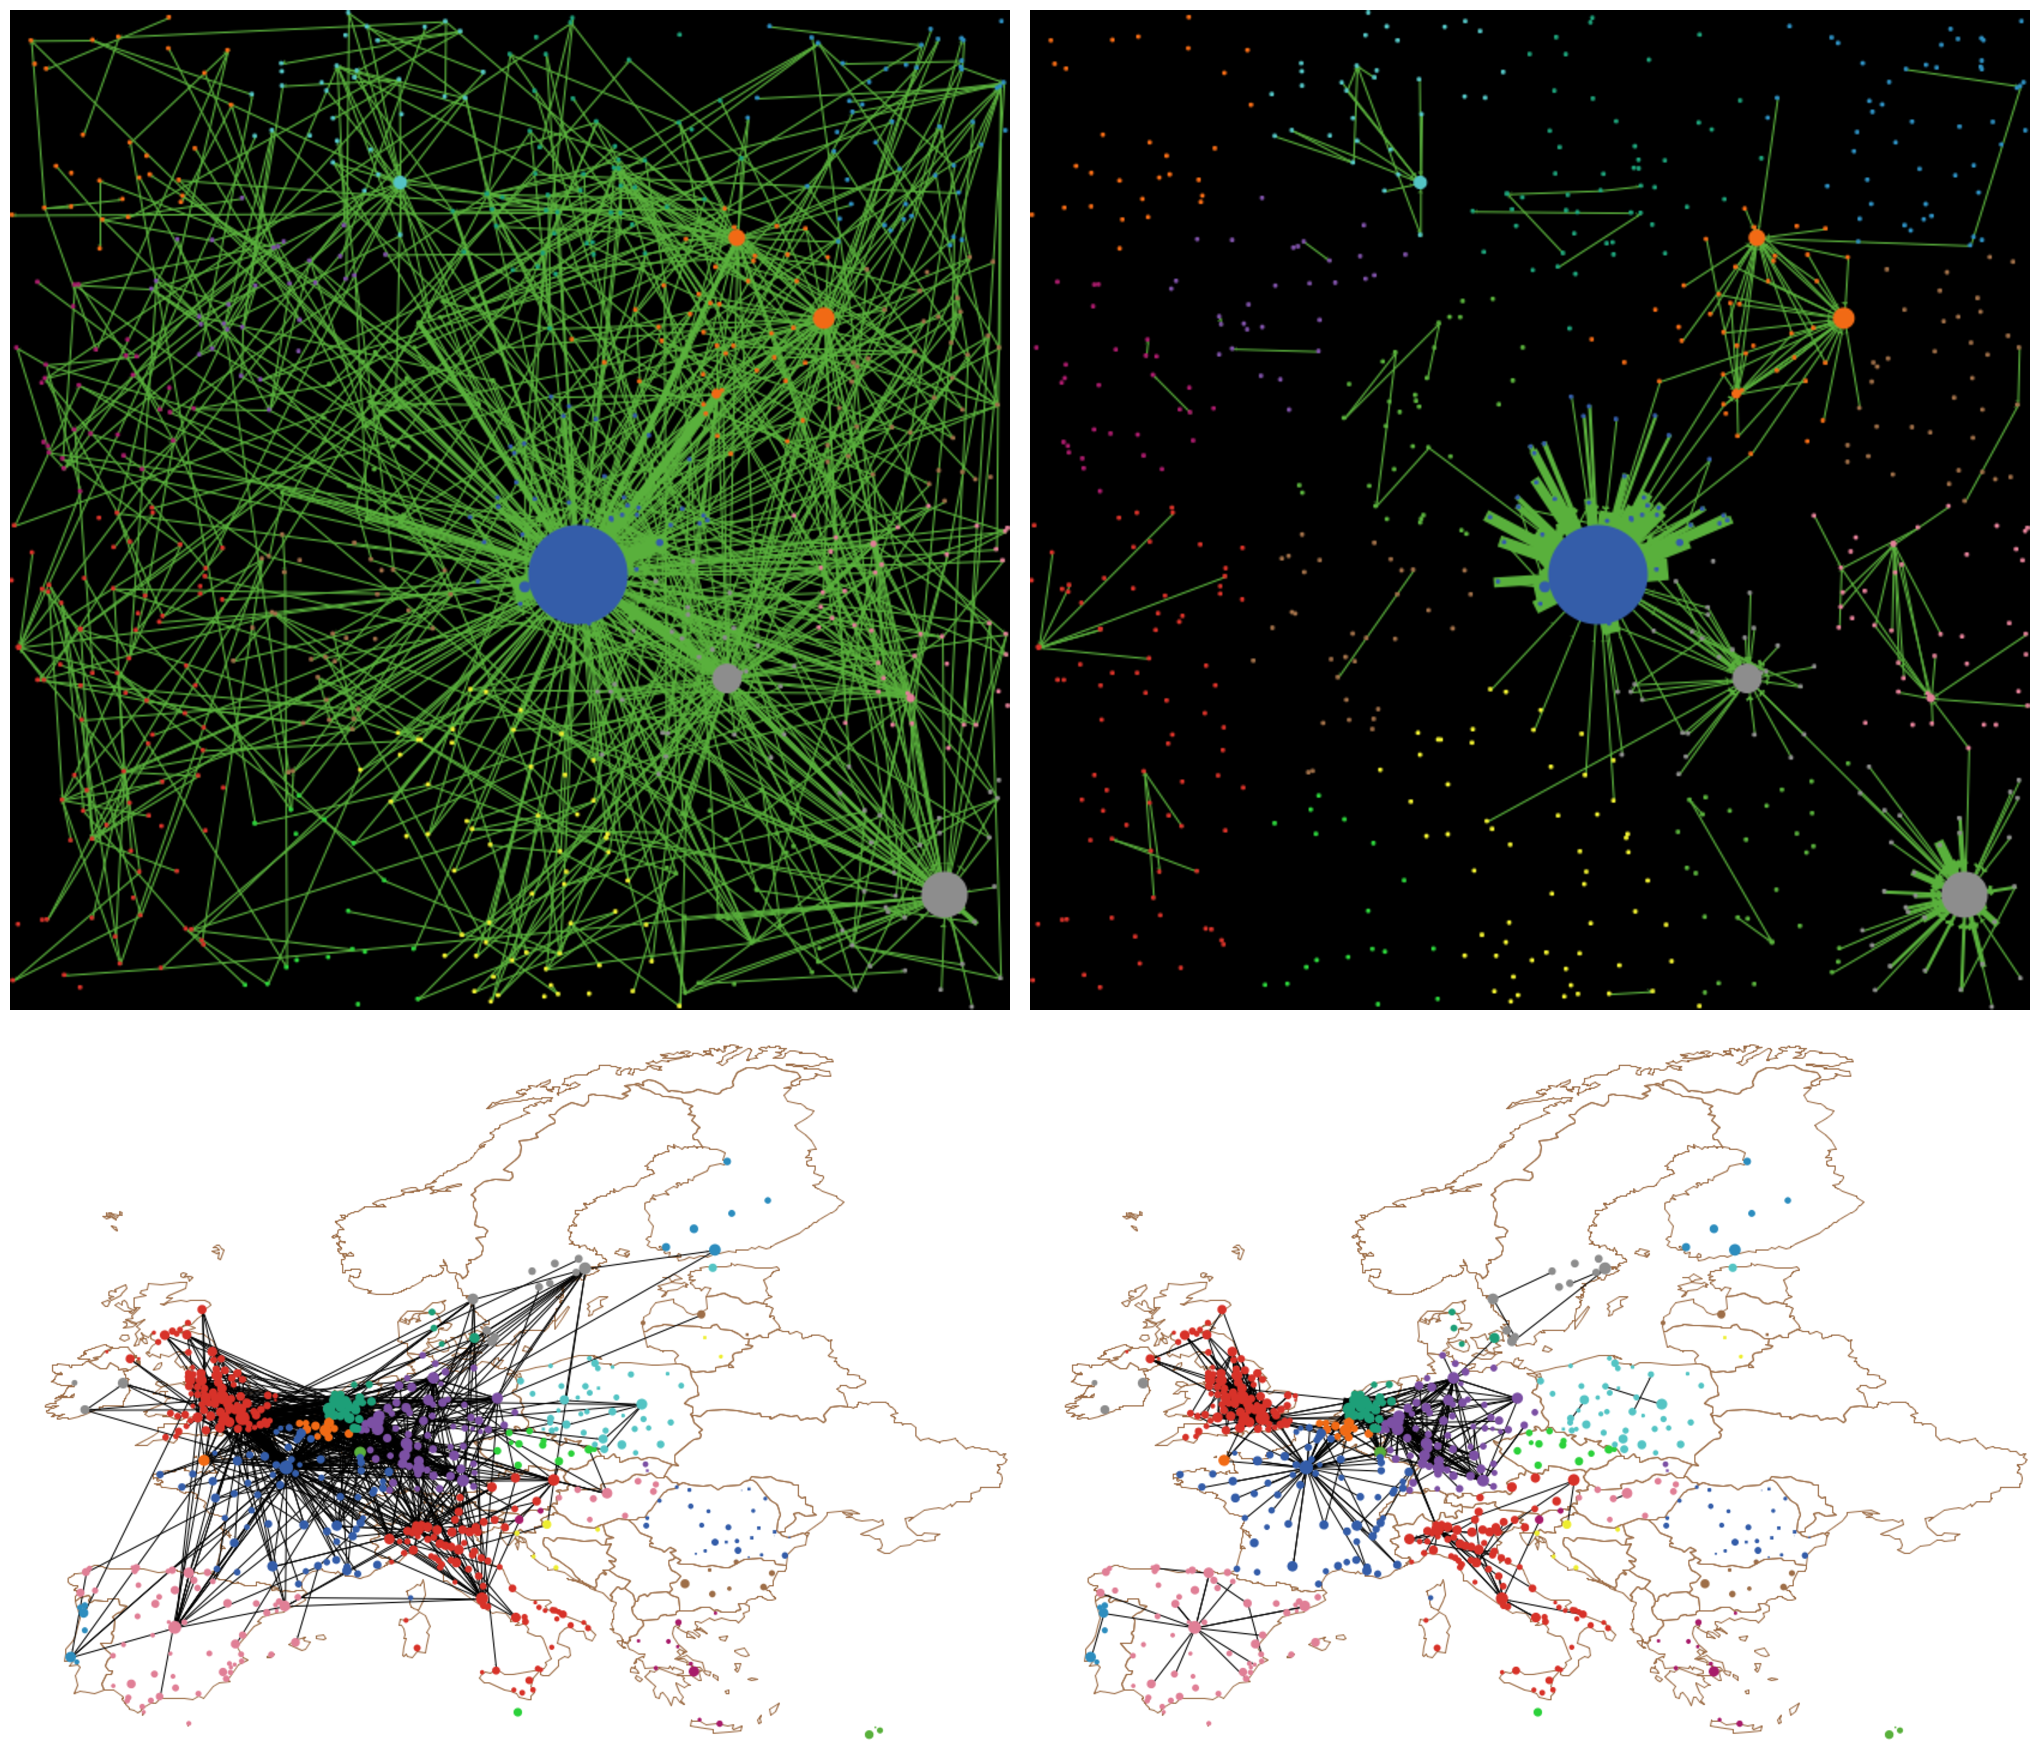
\includegraphics[width=0.67\textwidth]{../../figures/Fig3.png}
 \end{center}

\footnotesize

	\textit{Simulated networks in a synthetic setup (top) and real setup (bottom), for a large (resp. low) interaction range $d_0$ (left, resp. right).}

}


\sframe{Effect of interaction decay}{
    
    % One factor sampling results
    %  20190924_162740_ONEFACTOR_REPLICATIONS_SYNTHETIC_GRID
    
    \includegraphics[width=0.48\textwidth]{../../figuresraw/internationalisation-gravityDecay_errorbars.png}
    \includegraphics[width=0.48\textwidth]{../../figuresraw/metropolisation-gravityDecay_errorbars.png}
    
    \medskip
    
    \footnotesize
    
    \textit{(Left) Internationalization index decreases exponentially with gravity decay; (Right) Correlation between city weighted degree and size. Both plots show a transition from a local to a global regime.}
    
}


\sframe{Effect of sector proximity}{
    
    % One factor sampling results
    %  20190924_162740_ONEFACTOR_REPLICATIONS_SYNTHETIC_GRID
    
     \includegraphics[width=0.48\textwidth]{../../figuresraw/internationalisation-gammaSectors_errorbars.png}
    \includegraphics[width=0.48\textwidth]{../../figuresraw/metropolisation-gammaSectors_errorbars.png}
    
    \medskip
    \footnotesize
    
    \textit{(Left) Internationalization varies linearly with sector proximity $\gamma_S$; (Right) Correlation between degree and size exhibits a maximum, witnessing an intermediate regime where size is the most important}
    
    
}


\sframe{Grid exploration: internationalization}{

    \begin{center}
    \includegraphics[width=\textwidth]{../../figures/Fig5.png}
    \end{center}
    
    \medskip
    
    \footnotesize
    
    \textit{The transition as a function of interaction range depends on the influence of origin size $\gamma_F$; sector proximity $\gamma_S$ plays a role only for a large influence of the origin.}
    
}

\sframe{Grid exploration: community size}{

    \begin{center}
    	\includegraphics[height=0.6\textheight]{../../figures/Fig6.png}
    	
    \end{center}
    
    \vspace{-0.5cm}
    
    \footnotesize

\begin{itemize}
	\item Maximal integration in term of community size is achieved at an intermediate value of $d_G$: emergence of a regional regime
	\item Maximal size depends on the role of sectors $\gamma_S$, in a decreasing way when origin size is deactivated, and increasing way when $\gamma_F=1$
	\item This regime disappear when origin size influence is too large
\end{itemize}
    
}


\sframe{Calibration on the European urban network}{

    \begin{center}
    	\includegraphics[height=0.75\textheight]{../../figures/Fig8.png}
    	
    \end{center}
    
    \footnotesize
    
\textit{Pareto front obtained for the bi-objective model calibration using a NSGA2 algorithm (outperforms statistical models that have a MSE of 5.33).}

    
}


\sframe{Economic shock scenarios}{

    \begin{center}
    	\includegraphics[height=0.72\textheight]{../../figures/Fig9.png}
    	
    \end{center}
    
    %\vspace{-0.5cm}
    
    \footnotesize

\textit{Although the system is resilient to moderate shocks, strong restrictions have an important impact on internationalization and thus can be
expected to have a detrimental effect on UK economy due to these foreign ownership links.}
    
}


\section{Discussion}

\sframe{Discussion}{

\justify

\textbf{Practical application}

\medskip

$\rightarrow$ Potential application to public policy issues;

$\rightarrow$ Effect of exogenous shocks on specific economic sectors mostly dependent on foreign ownership links (extraction of crude petroleum, manufacture of tobacco \& basic pharmaceutical goods, activities of head offices).

\bigskip

\textbf{Developments}

$\rightarrow$ co-evolution model (evolution of city sizes) \cite{raimbault2018modeling};

$\rightarrow$ a model with firm agents (multi-scale ABM) \cite{raimbault:halshs-02351722};

$\rightarrow$ targeted study of path dependency;

$\rightarrow$ other formulation of the combination of factors or multi-objective optimisation depending on sectors using Pareto fronts.


}


\sframe{Conclusion}{

$\rightarrow$ A generative model to understand processes of economic network emergence

\bigskip

$\rightarrow$ Crucial role of model exploration to validate and extract knowledge from such a simulation model


\bigskip
\bigskip

\textbf{Preprint at} \texttt{https://arxiv.org/abs/2009.05528}

\bigskip

\textbf{Open repository for model and results at}

\texttt{https://github.com/JusteRaimbault/ABMCitiesFirms}

\bigskip

\textbf{Simulation data at} \texttt{https://doi.org/10.7910/DVN/UPX23S}

\bigskip

\textbf{Acknowledgments}: thanks to the \textit{European Grid Infrastructure} for access to the infrastructure. We also acknowledge the funding of the EPSRC grant EP/M023583/1


}



%%%%%%%%%%%%%%%%%%%%%
\begin{frame}[allowframebreaks]
\frametitle{References}
\bibliographystyle{apalike}
\bibliography{biblio}
\end{frame}
%%%%%%%%%%%%%%%%%%%%%%%%%%%%



\sframe{Reserve slides}{

\Huge

\centering

Reserve slides

}

\sframe{Empirical network properties}{

\begin{center}
    \includegraphics[width=\linewidth]{../../figures/Fig1.png}
\end{center}

\textit{Empirical distribution of network properties, with log-normal and power law fits}

}

\begin{frame}[label=syntheticsetup]

\frametitle{Synthetic setup}

\begin{enumerate}
    \item Generate $N \textrm{ = } 700$ cities with size following a power law $E_i \textrm{ = } E_0 \cdot i^{-\alpha}$ with $E_0 \textrm{ = } 10^{11}$ and $\alpha \textrm{ = } 1.1$ (computed on Europe for GDP with cities larger than 50.000 inhabitants)
    \item Distribute them randomly in space (\cite{simini2019testing} vs \cite{banos2011christaller})
    \item Create countries with k-means clustering ($C \textrm{ = } 30$)
    \item Distribute sectors such that (i) smaller cities are more specialized and (ii) larger cities are more knowledge-based, with a one dimensional axis to position sectors $1/K \ldots 1$ where the density $f\left(k\right)$ follows a log-normal with $\left(\mu,\sigma\right)$ such that $\sqrt{\Var f} \textrm{ = } K/2$ for the largest, $\sqrt{\Var f} \textrm{ = } 1/K$ for the smallest
\end{enumerate}

\hyperlink{setupmain}{\beamerbutton{Back}}

\end{frame}


\sframe{Global sensitivity analysis}{


\begin{center}
\resizebox{\linewidth}{!}{
    \begin{tabular}{|l|c|c|c|c|c|c|c|c|c|c|c|c|}
\hline
 & \multicolumn{2}{|c|}{$d_0$} & \multicolumn{2}{|c|}{$c_0$} & \multicolumn{2}{|c|}{$\gamma_S$} & \multicolumn{2}{|c|}{$\gamma_W$} & \multicolumn{2}{|c|}{$\gamma_O$} & \multicolumn{2}{|c|}{$\gamma_D$} \\
 & F & T & F & T & F & T & F & T & F & T & F & T \\
 \hline
Internationalisation & 0.2 & 0.3 & 0.7 & 0.7 & 0.001 & 0.009 & $4\cdot 10^{-4}$ & 0.007 & 0.03 & 0.04 & 0.02 & 0.04 \\
Metropolisation & 0.02 & 0.1 & 0.02 & 0.2 & 0.002 & 0.1 & 0.001 & 0.09 & 0.2 & 0.6 & 0.3 & 0.6 \\
Modularity & 0.3 & 0.4 & 0.6 & 0.6 & 0.004 & 0.02 & $3\cdot 10^{-4}$ & 0.01 & 0.005 & 0.03 & 0.002 & 0.03 \\
Avg. com. size & 0.008 & 0.09 & 0.01 & 0.1 & 0.002 & 0.07 & 0.003 & 0.04 & 0.3 & 0.6 & 0.4 & 0.6 \\
Degree entropy & 0.006 & 0.02 & 0.003 & 0.02 & 0.006 & 0.03 & 0.008 & 0.02 & 0.5 & 0.5 & 0.5 & 0.5 \\
Weight entropy & 0.04 & 0.1 & 0.03 & 0.1 & 0.008 & 0.08 & 0.01 & 0.07 & 0.4 & 0.5 & 0.4 & 0.5 \\\hline
\end{tabular}
}
\end{center}

\medskip

\textit{First order and total sensitivity indices \cite{saltelli2010variance}, for all parameters and indicators.}

}

\sframe{Role of urban hierarchy}{

\begin{center}
    \includegraphics[width=\linewidth]{../../figures/Fig7.png}
\end{center}

\medskip

\textit{Impact of urban hierarchy on model indicators in synthetic systems of cities.}

}





\end{document}

